%%%%%%%%%%%%%%%%%%%%%%%%%%%%%%%%%%%%%%%%%%%%%%%%%%%%%%%%%%%%%%%%%%%%%%%%
\clearpage
\section{Generalized form factor compliant for Titchmarsh transform }
\label{sect:TitchmarshObjects}
This generalized form factor include several special shapes like uniform spheres, spheres in Fraunhofer limit, thin randomly oriented platelets, long randomly oriented cylinder, etc.\ \cite{Fedorova1978}. A list of shapes is given in table \ref{tab:gFF}. They all have in common, that they only depend on one size parameter $a$. The parameter $\gamma$ additionally allows that scattering object contain other size parameters which must, however, be out of the $q$-range of the SAS experiment.

\begin{table}[htb]
\centering
\caption{Explicit expressions for $\displaystyle I(q)=\frac{1}{q^\gamma}\frac{J_\nu^2(qa)}{(qa)^\beta} \left(V_0a^\alpha\right)^2$ for several particle shapes. The values $n=\beta+1$ and $m=2\alpha-n$ where needed for the Titchmarsh transform in the paper from Fedorova}
\label{tab:gFF}
\begin{tabular}{|lL{5.5cm}|l|l|l|l|l|l|l|l|l|l|}
 \rowcolor[gray]{0.8}
\toprule
& shape
             & $I(q)/V_0^2$  & $\nu$ & $\gamma$ & $\beta$ & $n$ & $m$     & $\alpha$ & $s$ & $p$ & $d$\\ \midrule
1.& uniform sphere
             & $\displaystyle \frac{J^2_{3/2}(qa)}{(qa)^3} a^6$     & $\frac32$ & 0 & 3 & $4$  & $2$    & 3 & 0 & 4 & 3\\
 \rowcolor[gray]{0.95}
\parbox{0.3cm}{2.\newline\phantom{2.}}& Long cylinder perpendicular to
the plane of scattering
             &                                                       &            & & & & &          &   &   &   \\
 \rowcolor[gray]{0.95}
3.& Thin disc in scattering  plane
             & $\displaystyle \frac{J^2_{1}(qa)}{(qa)^2} a^4$        & 1  & 0     & 2 & 3 & 1                      & 2 & 0 & 3 & 2 \\
 \rowcolor[gray]{0.95}
\parbox{0.3cm}{4.\newline\phantom{4.}}& Sphere (Fraunhofer diffraction)
             &                                                       &            & & & & &           &   &   &  \\
\parbox{0.3cm}{5.\newline\phantom{5.}}  &Long randomly oriented cylinder
             & $\displaystyle \frac1q \frac{J^2_{1}(qa)}{(qa)^2} a^4$     & 1 & 1 & 2 & 3 & 1 & 2 & 1 & 4 & 3\\
 \rowcolor[gray]{0.95}
6.& Spherical shell
             & $\displaystyle \frac{J^2_{1/2}(qa)}{qa} a^4$          & $\displaystyle\frac12$ & 0 & 1 & 2 & 2 & 2 & 0 & 2 & 2 \\
\parbox{0.3cm}{7.\newline\phantom{7.}}& Thin randomly oriented
platelet
             & $\displaystyle \frac{1}{q^2}\frac{J^2_{1/2}(qa)}{qa} a^2$ & $\displaystyle\frac12$ & 2 & 1 & 4 & 0 & 1 & 2 & 4 & 3 \\
 \rowcolor[gray]{0.95}
\parbox{0.3cm}{8.\newline\phantom{8.}}& Long cylinder (Fraunhofer diffraction)
             & $\displaystyle \frac1q \frac{J^2_{1/2}(qa)}{qa} a^2$      & $\displaystyle\frac12$ & 1 & 1 & 3 & 0 & 1 & 1 & 3 & 2  \\
\parbox{0.3cm}{9.\newline\phantom{9.}\newline\phantom{9.}}& Thin rod perpendicular to the incident beam and in the plane of scattering
             & $\displaystyle \frac{J^2_{1/2}(qa)}{qa} a^2$       & $\displaystyle\frac12$ & 0 & 1 & 2 & 0  & 1 & 0 & 2 & 1\\
 \rowcolor[gray]{0.95}
\parbox{0.3cm}{10.\newline\phantom{10.}}& Hollow cylinder perpendicular to beam
             & $\displaystyle J^2_{0}(qa) a^2$      & 0   & 0  & 0 & 1 & 1 & 1 & 0 & 1 & 1\\
\parbox{0.3cm}{11.\newline\phantom{11.}}& Randomly oriented long hollow cylinder
             & $\displaystyle \frac1qJ^2_{0}(qa) a^2$     & 0  & 1 & 0 & 2 & 1 & 1 & 1 & 2 & 2 \\ \bottomrule
\end{tabular}

\end{table}

The generalized form factor is defined as
\begin{align}\label{eq:generalizedFF}
  I(q) &=  \frac{1}{q^\gamma}\frac{J_\nu^2(qa)}{(qa)^\beta} \left(V_0a^\alpha\right)^2 \\
       &=  \frac{1}{q^\gamma}\frac{\left(V_0a^{\alpha}\right)^2 4^{-\nu }}{(a q)^{\beta-2 \nu}\Gamma (\nu +1)^2} {}_0^{\phantom{2}}F^2_1\left(\{\},\{\nu+1\};-(qa)^2/4\right)
\end{align}
in the limits of $q\rightarrow 0$ and $q\rightarrow \infty$ the scattering intensities become
\begin{align}\label{eq:generalizedFFlimits}
\lim_{q\rightarrow 0}      I(q) & = \frac{1}{q^\gamma}\frac{\left(V_0a^{\alpha}\right)^2}{(a q)^{\beta -2\nu}}\frac{4^{-\nu }}{\Gamma (\nu +1)^2} \\
\lim_{q\rightarrow \infty} I(q) & = \frac{1}{q^\gamma}\frac{\left(V_0a^{\alpha}\right)^2}{\pi(aq)^{\beta+1}}
\end{align}
The parameter $\gamma$ is not necessarily required and any value of it could be replaced by a proper correction of the values for $\alpha$ and $\beta$. However, the parameter $\alpha$ was introduced to describe how the volume of the objects on which small angle scattering is sensitive scales with the parameter $a$. For a homogeneous cylinder oriented randomly with its radius in the range of the SAS experiments the object dimension is $d=3$. However, for an oriented cylinder where SAS is measured perpendicular to the cylinder axis the signal only probes the cross section and $d$ is therefore 2. If $a$ is the smaller or larger dimension of an very anisotropic object like thin local cylindrical objects or thin local planar objects the volume scales with $V_0a^\alpha l^\gamma$ where $l\gg a$ or $l\ll a$ describes the larger or smaller dimensions of the object. The overall dimension of the object is $1\leq d=\alpha+\gamma\leq3$ and should lay between 1 and 3. Furthermore the overall dimension $d$ of the object needs to be larger than $\alpha$, i.e $2\geq\gamma\geq 0$. As only the dimension $a$ is probed in the case of $l\gg a$ the larger dimension $l$ leads to a potential law behaviour at small $q$-values with $s=\gamma$. This is an additional constrain leading to the lesser generalized form factor having three input parameters either $(d,s,p)$ or $(d,\alpha,p)$.
\begin{align}\label{eq:lesser_generalizedFFparameters}
\begin{array}{rl}
  s &= \gamma \\
 s &= \gamma + \beta -2\nu \\
 p &= \gamma+\beta+1 \\
 d &= \alpha+\gamma
\end{array}
\Rightarrow
\begin{array}{rl}
 \alpha &= d-s \\
 \beta &= p-s-1 \\
 \gamma &= s \\
 \nu &=\beta/2
\end{array}
\Leftrightarrow
\begin{array}{rl}
 s &= d-\alpha \\
 \beta &= \alpha+p-d-1 \\
 \gamma &= s \\
 \nu &=\beta/2
\end{array}
\end{align}
The other constrains on the parameters for physical meaningful two-phase models with sharp interfaces are $(3\geq d\geq \alpha\geq 1)$,  $(2\geq s\geq 0)$, $(4\geq p \geq 1)$, $(\beta,\nu\geq 0)$.

\vspace{5mm}

\underline{Input Parameters for model \texttt{generalized form factor}:}\\
\begin{description}
\item[\texttt{a}] size parameter $a$
\item[\texttt{sigma\_a}] width $\sigma_a$ of the size distribution (LogNorm)
\item[\texttt{alpha}] dimensionality parameter $\alpha$ related to $a$.
\item[\texttt{beta}] decay at large scattering vectors, $q^p$, with $p=\gamma+\beta+1$
\item[\texttt{gamma}] additional potential law $q^\gamma$
\item[\texttt{nu}] shape parameter $\nu$
\item[\texttt{eta}] scattering length density contrast $\Delta\eta$
\end{description}

\vspace{5mm}

\underline{Input Parameters for model \texttt{lesser generalized form factor 1}:}\\
\begin{description}
\item[\texttt{a}] size parameter $a$
\item[\texttt{sigma\_a}] width $\sigma_a$ of the size distribution (LogNorm)
\item[\texttt{alpha}] dimensionality parameter $\alpha$ related to $a$.
\item[\texttt{dummy}] not used
\item[\texttt{s}] potential law at small $q$-values
\item[\texttt{p}] potential law at large $q$-values
\item[\texttt{eta}] scattering length density contrast $\Delta\eta$
\end{description}

\vspace{5mm}

\underline{Input Parameters for model \texttt{lesser generalized form factor 2}:}\\
\begin{description}
\item[\texttt{a}] size parameter $a$
\item[\texttt{sigma\_a}] width $\sigma_a$ of the size distribution (LogNorm)
\item[\texttt{dummy}] not used
\item[\texttt{dim}] overall dimension $d$ of the particle ($1\leq d\leq 3$)
\item[\texttt{s}] potential law $q^{-s}$ at small $q$-values
\item[\texttt{p}] potential law $q^{-p}$ at large $q$-values
\item[\texttt{eta}] scattering length density contrast $\Delta\eta$
\end{description}

\vspace{5mm}

\underline{Note:}
\begin{itemize}
\item $(3\geq d\geq \alpha\geq 1)$
\item $(2\geq s\geq 0)$
\item  $(4\geq p \geq 1)$
\item $(\beta,\nu\geq 0)$.
\end{itemize}

\begin{figure}[hbt]
\begin{center}
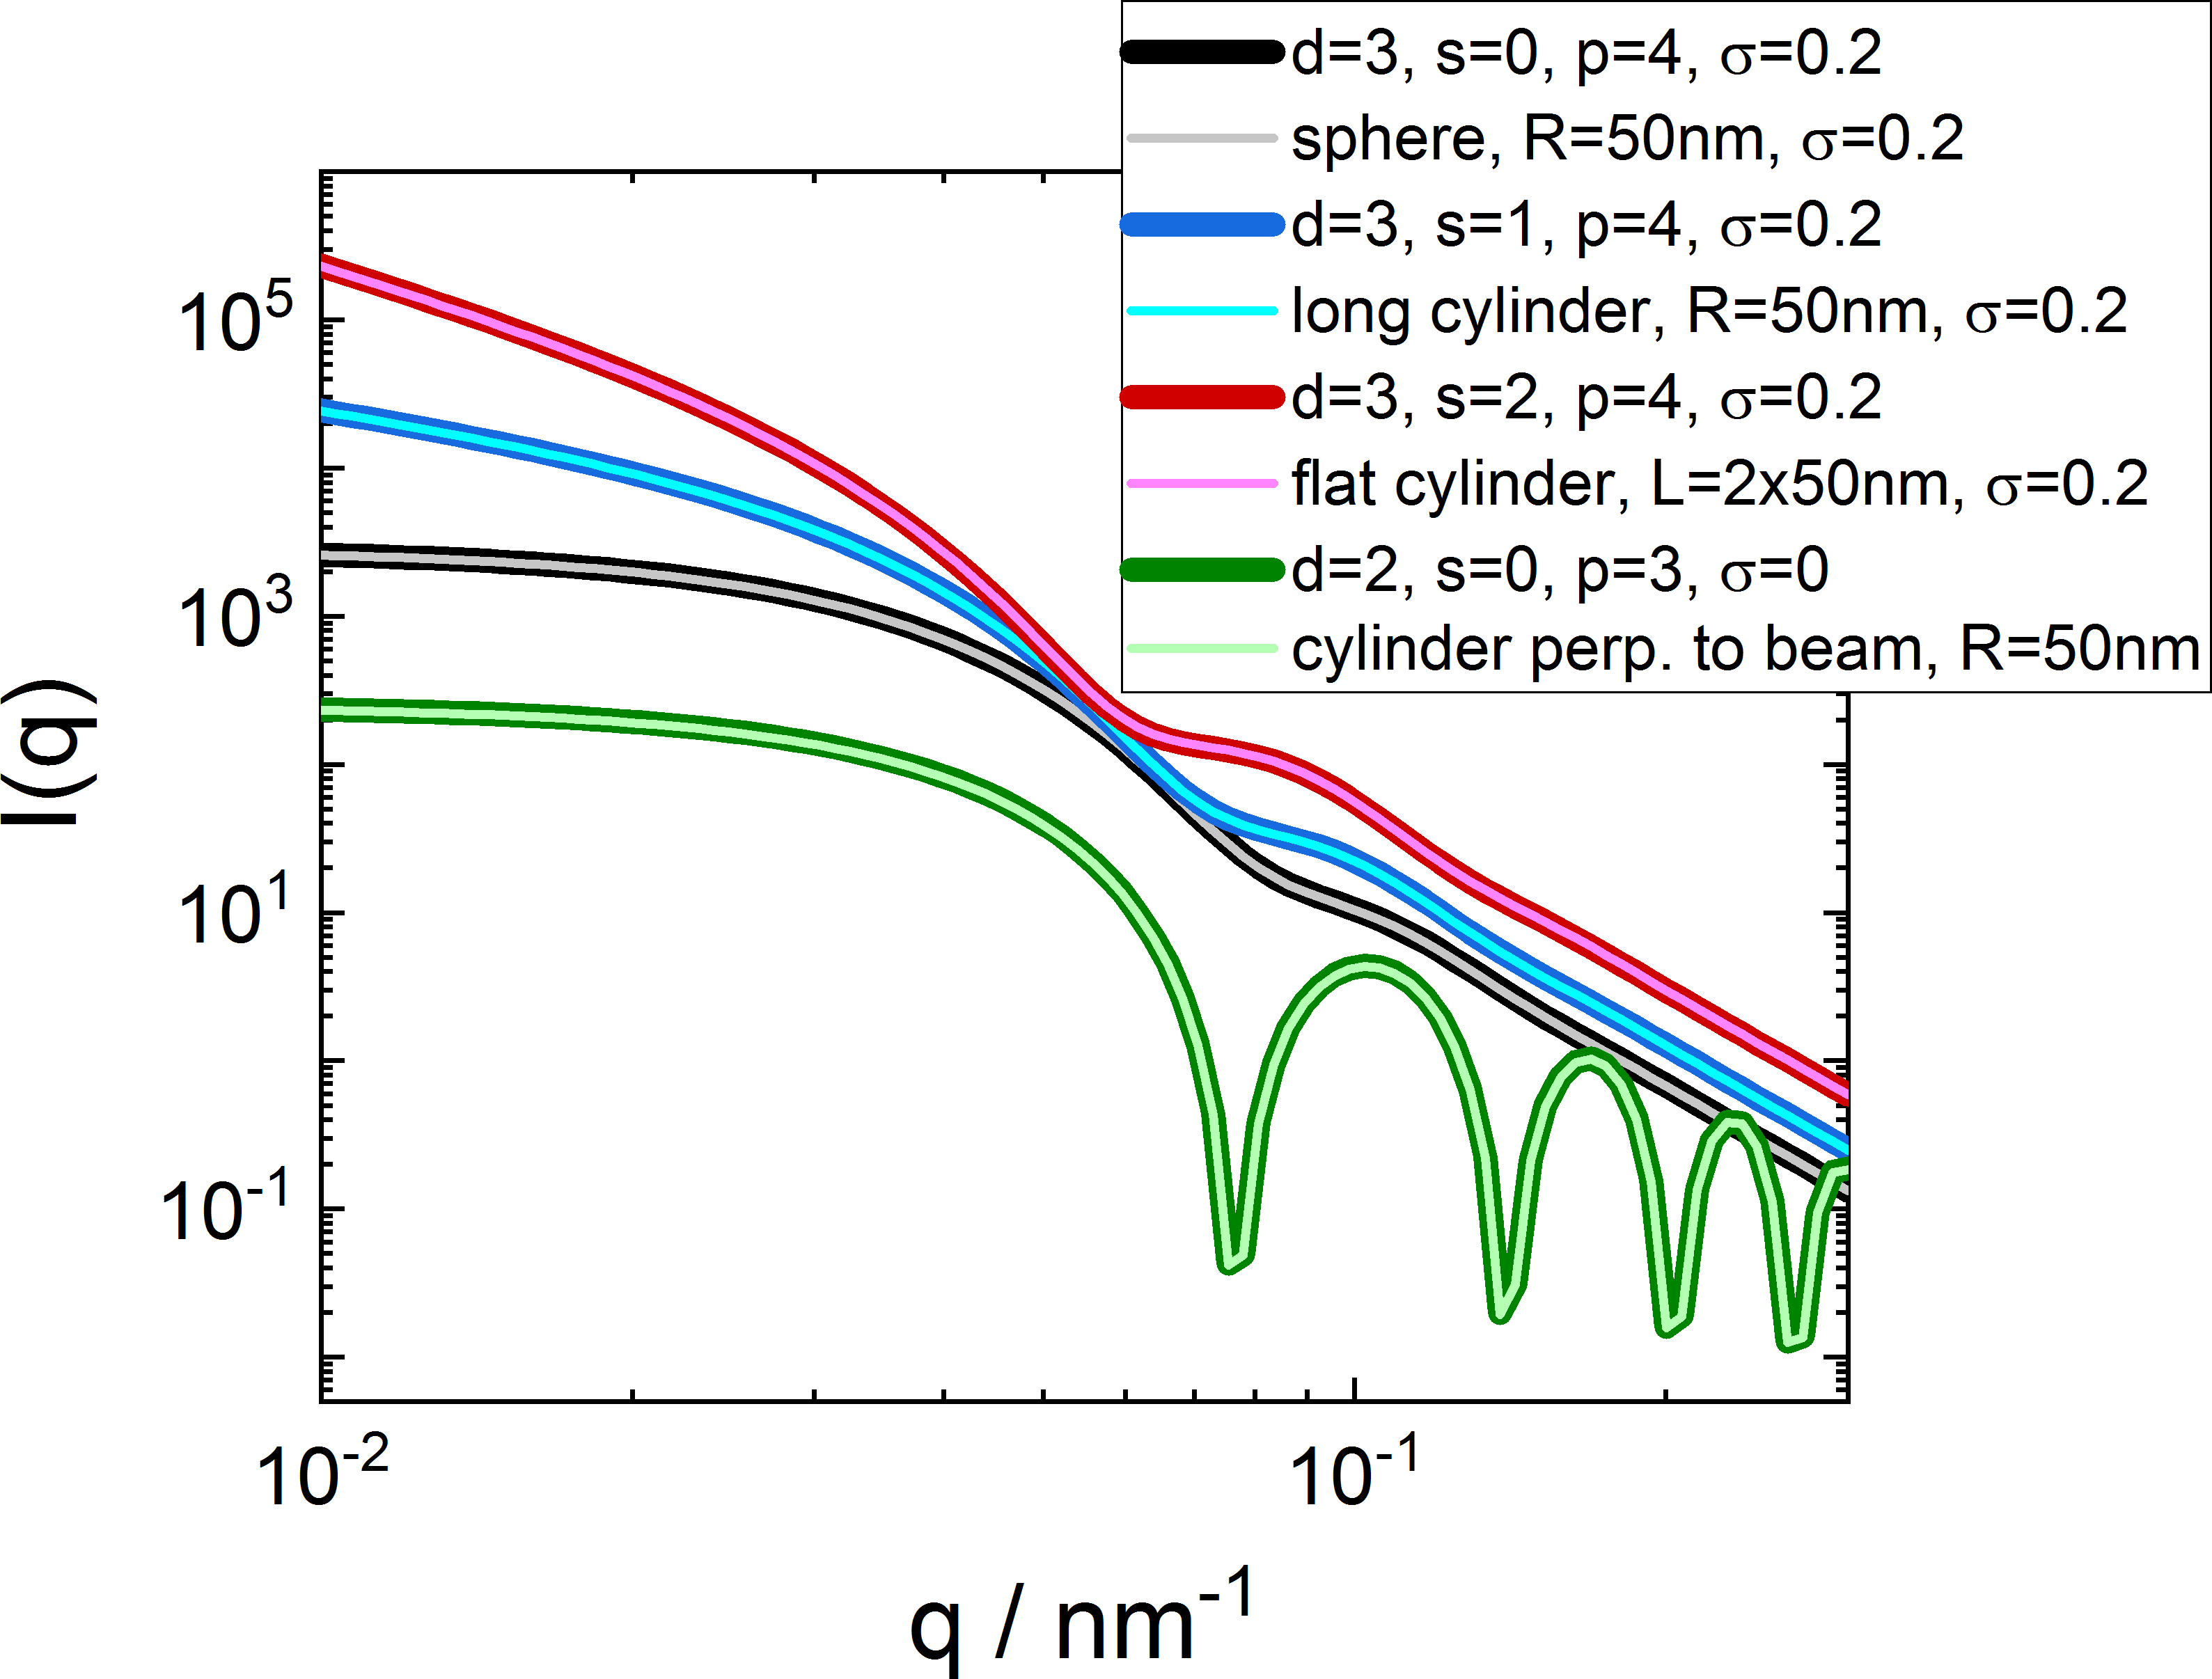
\includegraphics[width=0.75\textwidth]{../images/form_factor/gFF/gFF.png}
\end{center}
\caption{Comparison of generalized form factor with certain geometries namely \texttt{Sphere}, \texttt{LongCylinder}, \texttt{FlatCylinder}, \texttt{cylinder (OPO)} (cylinder perp. to beam).} \label{fig:gFFIQ}
\end{figure}